\subsection{Pump spot scalability}
\label{sec:eval:pumpspot}

One way to augment the output power
is to increase the pumped area
\cite{Tropper2006,Chernikov2010,Korpi2010}.
A power scalable device
would increase the output power
proportional to the irradiated area.
As described in section~\ref{sec:rth:scaling},
this ideal description
doesn't work for real VECSELs;
the lateral cooling
is important
after all
\cite{Chernikov2010}.

By investigating
the scaling behavior
we can learn about
the limits
of the performance
of our device.
We vary the pump spot size
using lenses with various focal lengths
in order to image the $200\,\mu\mathrm{m}$ diameter fiber
onto sample 1,
see section~\ref{sec:exp:setup}.
For the scaling experiments
I irradiated spot A
indicated in Fig.~\ref{img:sample_surface}.
Because of the change
of lens $\mathrm{L}_\mathrm{p2}$
and the subsequent
realignment of the setup,
I cannot ensure to have hit the exact same spot.
The employed cameras help us
to find it approximately,
but the remaining uncertainty is hard to estimate.
I imply the sample is homogeneous enough on this scale.
Each data point
is measured $N=3$ times.

\subsubsection{Output power}
\label{sec:eval:pumpspot:pwr}

In order to learn
about the scaling behavior
of the output power,
we look 
at the light-light characteristics
obtained from different
pump spot sizes.
Output scaling with area
only works up to a point,
above which
amplified spontaneous emission (ASE) losses
become significant
\cite{Hessenius2011}.
Bedford et al. \cite{Bedford2005}
also estimate
there to be
a critical diameter
above which lateral lasing
is likely to occur
before the intended
transversal lasing.
With our measurements,
we're interested
to see the experimental
scaling behavior
of our structure
for spot sizes
realistic in real world applications.

\begin{figure}
\centering
\subfigure{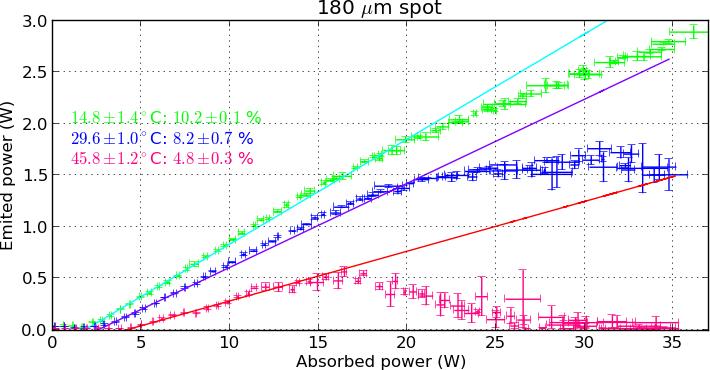
\includegraphics[width=14.5cm]{img/LL_spot180um.png}}
\subfigure{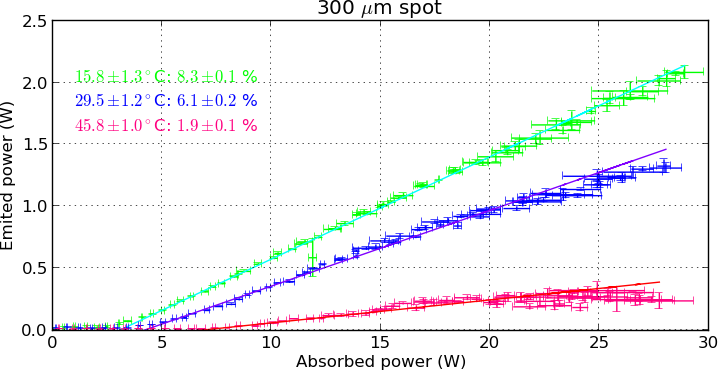
\includegraphics[width=14.5cm]{img/LL_spot300um.png}}
\subfigure{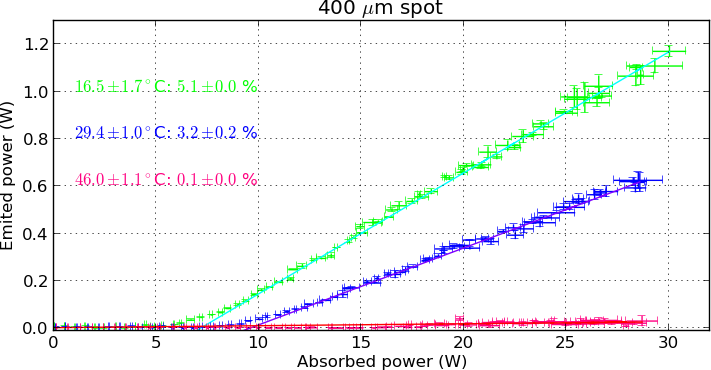
\includegraphics[width=14.5cm]{img/LL_spot400um.png}}
\caption{Light-light characteristics
for different spot sizes
obtained with spherical lenses.
The efficiency decreases
for increased spot size.
This may be due to
inefficient heat extraction
manifested in sub-area scaling of $\Rth$,
discussed in section~\ref{sec:eval:pumpspot:rth}.}
\label{img:LL_spot_scaling}
\end{figure}

Figure~\ref{img:LL_spot_scaling}
plots the resulted
light-light characteristics
for various spot sizes,
measured at the heat sink temperatures
$\{15,30,45\}\,^\circ\mathrm{C}$,
using spherical lenses
for both $\mathrm{L}_\mathrm{p1}$ and $\mathrm{L}_\mathrm{p2}$.
The average maintained heat sink temperature,
plus-minus its standard deviation,
is stated in each of the subplots,
accompanied by the slope efficiency
corresponding to
the straight lines.
The slope efficiency
is obtained
by taking into account
only the data points
of the linear segment.
The onset of
the roll over region
is ignored.

The most obvious conclusion
we can draw from these measurements
is that
our device is not power scalable:
the conversion efficiency
decreases for larger pump spots,
while in a scalable device
it should not.
Consequentially,
the maximally achieved
output power
is not increased
for larger pump spots.
In order to explain this
we acknowledge that
with larger pump spots
we're more likely
to hit non-radiative defects
\cite{Korpi2010}.
Secondly,
the thermal resistance
is empirically demonstrated
to decrease less efficiently
than with irradiated area.
The initial explanation
why VECSELs are expected
to power scale
relies on the one dimensional
heat extraction.
In reality
the contribution
of lateral cooling
must not be neglected
\cite{Chernikov2011}.

Beside the decrease
in conversion efficiency,
the roll over point
shifts to higher absorbed power
for larger pump spots.
This indicates
the structure
to heat up less
for larger pump spots.
The findings
concerning the thermal resistance
discussed in \ref{sec:eval:pumpspot:rth}
support this interpretation.

I performed
these scaling measurements
also with lens
$\mathrm{L}_\mathrm{p1}$
replaced by
an achromatic lens.
We would not assume
to find significant
differences
in the scaling behavior
since the spectral profile
of our pump source
is fairly narrow,
Fig.~\ref{img:pumpspectrum}.
Nevertheless,
this assumption needs to be tested.
Secondly,
these measurements yield
additional data points
for the thermal resistance
scaling behavior,
discussed in \ref{sec:eval:pumpspot:rth}.

The investigated spot diameters
are $\{222,333,444\}\,\mu\mathrm{m}$
for the achromatic configuration.
The used output coupler
is not optimal
for spot sizes larger than
$400\,\mu\mathrm{m}$.
The performance
corresponding to
the $444\,\mu\mathrm{m}$ spot
was indeed worse
than the one 
corresponding to
the $333\,\mu\mathrm{m}$ spot.
However,
the $222\,\mu\mathrm{m}$ spot
performed even worse.
Given this discrepancy,
I have to discard
the results
from the spot scaling experiments
in the achromatic setting.
Non the less,
all of these three measurements
showed an improved performance
with respect to
the spherical lens configuration.

We don't know the exact beam shape,
and the estimation
of the spot size
is the result
of a ray optical consideration.
The uncertainty
resulting from this approach
should be looked into more closely
in future investigations.
The fact that the pump beam shape
is relevant
was demonstrated
in \cite{Chernikov2010}.
The improved output performance
seen in our setup,
by simply changing
the type of
one of the pump delivery lenses,
also indicate
on the importance
of the pump profile.
A summary on beam shape alteration
is given
in appendix~\ref{app:spatial}
and \cite{Mansell2000}. 

For now we can only speculate
why incorporating
the achromatic lens
improves the output performance
the way it did.
I investigated
the $333\,\mu\mathrm{m}$ configuration
more thoroughly.
The results were
reproducible and thus credible.
The measurements
concerning the proposed improvements
\cite{Hader2011}
presented in section~\ref{sec:eval:maxout},
were obtained in this configuration.
\subsubsection{Thermal resistance}
\label{sec:eval:pumpspot:rth}

In order to determine the thermal resistance $\Rth$
we have to look at
the longest emitted wavelength $\lambda$
at different heat sink temperature
versus dissipated power $D$,
(\ref{eq:dissip}).
According to the method
described in section~\ref{sec:rth:lambda}
we can find a linear relation
between $\lambda$ and $D$,
from which we can deduce
the thermal resistance $\Rth$.
We do this
for the different spot sizes,
and can thus conclude
on the scaling behavior.

The spot sizes
$\{180,300,400\}\,\mu\mathrm{m}$
were each measured for the temperatures
$\{15,30,45\}\,^\circ\mathrm{C}$,
using spherical lenses
for both $\mathrm{L}_\mathrm{p1}$ and $\mathrm{L}_\mathrm{p2}$,
as described in section~\ref{sec:exp:setup}.
Figure~\ref{img:Rth_lambda_spot_scaling}
plots the resulted longest wavelengths
against dissipated power.
The average maintained heat sink temperature,
plus-minus its standard deviation,
is stated in each of the subplots.
The straight lines correspond
to the linear fit (\ref{eq:rth_fit}).
The inset text in black
takes note of this fit,
displaying the fit parameters in values.
The stated thermal resistance results from
the ratio of the two fit parameters (\ref{eq:rth_long})
\begin{equation*}
\Rth = \pd{T}{D} = \pd{\lambda}{D}/\pd{\lambda}{T}.
%\label{eq:rth_long}
\end{equation*}

In order to obtain the fit
we consider only the data points
corresponding to
the linear light-light conversion regime --
the same as for estimating
the conversion efficiency
in section~\ref{sec:eval:pumpspot:pwr},
Fig.~\ref{img:LL_spot_scaling}.
This means
we exclude both,
threshold
and roll over segments.

Figure~\ref{img:Rth_spotsizescaling}
shows the scaling of $\Rth$
with respect to spot size.
The plot to the left
displays the behavior
noted in \cite{Giet2008}
and highlighted
in section~\ref{sec:rth:scaling}:
the thermal resistance
decreases less efficiently
than by area.
The reduction in $\Rth$
is closer to $w^{-1}$
than $w^{-2}$,
as illustrated
by the slope
given in the log-log plot.

A VECSEL device is thin
compared to the pumped area.
The expected heat flow
is one dimensional,
independent on lateral cooling.
The observed scaling behavior
shows this approximation
is not tenable.
In an attempt to understand
this behavior
when we look at
the expected temperature profile
from Fig.~\ref{img:Comsol_Tvsr}.
The temperature peaks
at the center
in the case of the depicted Gauss
and super-Gaussians and,
consequentially,
lateral heat transfer occurs,
beside the one-dimensional extraction
\cite{Chernikov2011}.

The measurements conducted
with the achromatic lens
could not be used
to extract the thermal resistance
with the method described
in section~\ref{sec:rth:lambda}.
Fit (\ref{eq:rth_fit}) relies
on a linear relation
between $\lambda$ and $D$
\cite{Heinen2012}.
As will be discussed
in section~\ref{sec:eval:trollover},
Fig.~\ref{img:lambda_sample},
this linearity was not given.

The fit in turquoise
corresponds to (\ref{eq:Rth_empirical}).
With only three data points available
to fit three parameters
we cannot judge
how good the found parameters
actually are.
But given the original meaning
of $a_3$ --
an outer radius  of a VCSEL --
we recognize the found values
not to make too much sense.
The found fit is valid
only for spot sizes smaller
than $2w=550\,\mu\mathrm{m}$.
This,
together with the large uncertainties
attached to the estimates of the thermal resistance,
show there needs more work to be done
in order to get a useful statement
out of the analysis of $\Rth$.


\begin{figure}
\centering
\subfigure{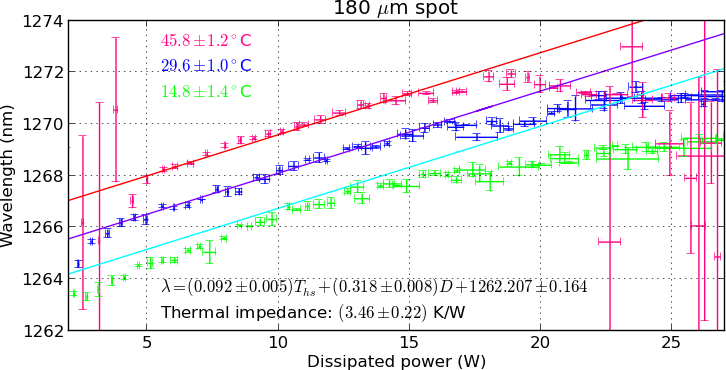
\includegraphics[width=14.5cm]{img/Rth_lambda_spot180um.png}}
\subfigure{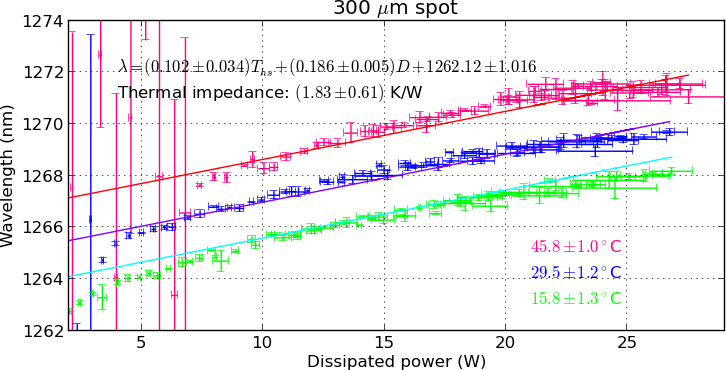
\includegraphics[width=14.5cm]{img/Rth_lambda_spot300um.png}}
\subfigure{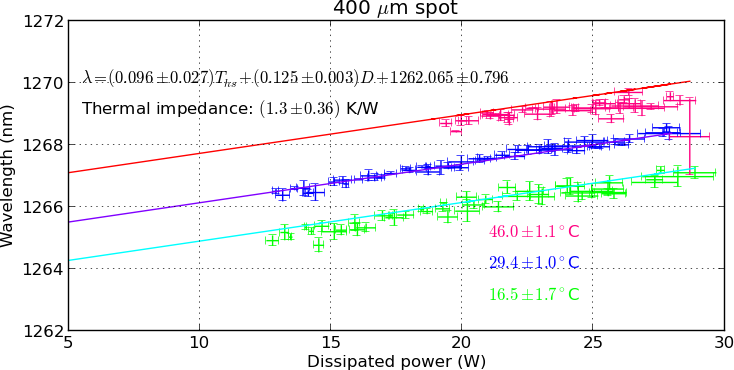
\includegraphics[width=14.5cm]{img/Rth_lambda_spot400um.png}}
\caption{Estimating $\Rth$ with
the method described in section~\ref{sec:rth:lambda}
for three pump spot sizes.
The straight lines correspond
to the fit (\ref{eq:rth_fit}),
taking into account
only the part of linear light-light conversion --
i.e. without the threshold
or roll over segments.}
\label{img:Rth_lambda_spot_scaling}
\end{figure}



\begin{figure}
\centering
\subfigure{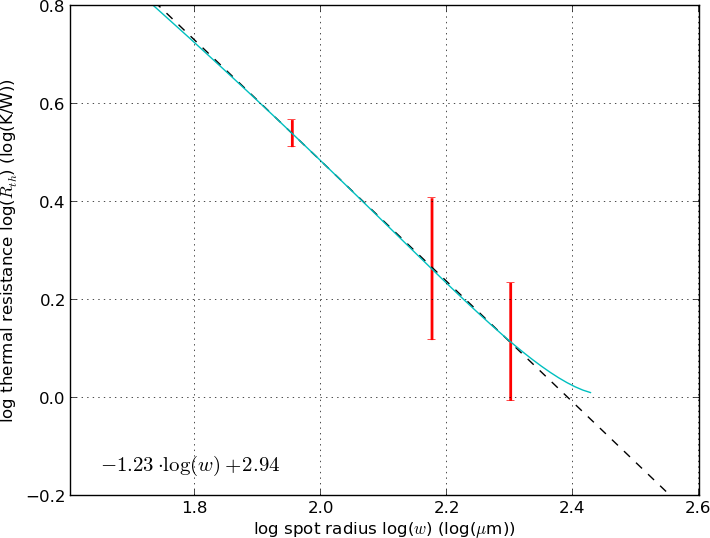
\includegraphics[width=7cm]{img/Rth_spotsizescaling_log.png}}
\subfigure{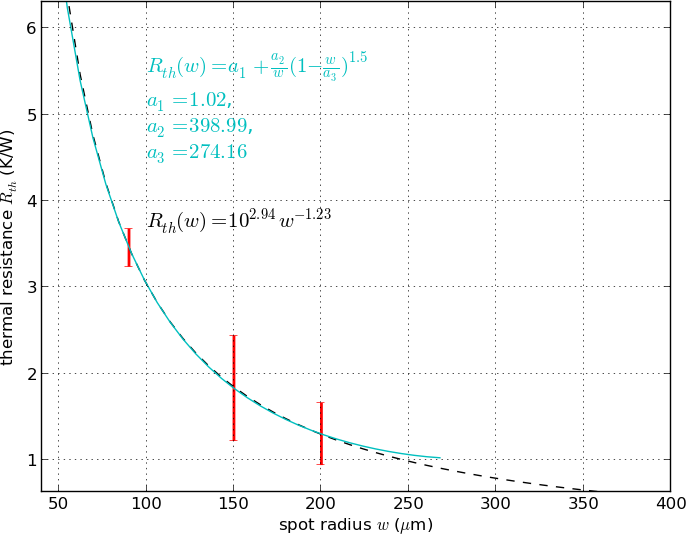
\includegraphics[width=7cm]{img/Rth_spotsizescaling_lin.png}}
\caption{Scaling of thermal resistance
(from Fig.~\ref{img:Rth_lambda_spot_scaling})
with spot size.
Its dependency on spot diameter is expected to be closer to
$(2w)^{-1}$ than $(2w)^{-2}$;
i.e. not to scale with area \cite{Giet2008}.
This is visualized by the slope in the log-log plot (left).
The continuous curve in turquoise shows a fit to
an empirical curve (\ref{eq:Rth_empirical}) \cite{Giet2008,Nakwaski1992}.
Right,
what the fits look like with linear axes.}
\label{img:Rth_spotsizescaling}
\end{figure}







